\documentclass[11pt,compress,t,notes=noshow]{beamer}\usepackage[]{graphicx}\usepackage[]{color}

\makeatletter
\def\maxwidth{ %
  \ifdim\Gin@nat@width>\linewidth
    \linewidth
  \else
    \Gin@nat@width
  \fi
}
\makeatother

\definecolor{fgcolor}{rgb}{0.345, 0.345, 0.345}
\newcommand{\hlnum}[1]{\textcolor[rgb]{0.686,0.059,0.569}{#1}}%
\newcommand{\hlstr}[1]{\textcolor[rgb]{0.192,0.494,0.8}{#1}}%
\newcommand{\hlcom}[1]{\textcolor[rgb]{0.678,0.584,0.686}{\textit{#1}}}%
\newcommand{\hlopt}[1]{\textcolor[rgb]{0,0,0}{#1}}%
\newcommand{\hlstd}[1]{\textcolor[rgb]{0.345,0.345,0.345}{#1}}%
\newcommand{\hlkwa}[1]{\textcolor[rgb]{0.161,0.373,0.58}{\textbf{#1}}}%
\newcommand{\hlkwb}[1]{\textcolor[rgb]{0.69,0.353,0.396}{#1}}%
\newcommand{\hlkwc}[1]{\textcolor[rgb]{0.333,0.667,0.333}{#1}}%
\newcommand{\hlkwd}[1]{\textcolor[rgb]{0.737,0.353,0.396}{\textbf{#1}}}%
\let\hlipl\hlkwb

\usepackage{framed}
\makeatletter
\newenvironment{kframe}{%
 \def\at@end@of@kframe{}%
 \ifinner\ifhmode%
  \def\at@end@of@kframe{\end{minipage}}%
  \begin{minipage}{\columnwidth}%
 \fi\fi%
 \def\FrameCommand##1{\hskip\@totalleftmargin \hskip-\fboxsep
 \colorbox{shadecolor}{##1}\hskip-\fboxsep
     \hskip-\linewidth \hskip-\@totalleftmargin \hskip\columnwidth}%
 \MakeFramed {\advance\hsize-\width
   \@totalleftmargin\z@ \linewidth\hsize
   \@setminipage}}%
 {\par\unskip\endMakeFramed%
 \at@end@of@kframe}
\makeatother

\definecolor{shadecolor}{rgb}{.97, .97, .97}
\definecolor{messagecolor}{rgb}{0, 0, 0}
\definecolor{warningcolor}{rgb}{1, 0, 1}
\definecolor{errorcolor}{rgb}{1, 0, 0}
\definecolor{code}{rgb}{0.97, 0.96, 1.0}
\newenvironment{knitrout}{}{} % an empty environment to be redefined in TeX

\usepackage{alltt}
\usepackage[utf8]{inputenc}
\usepackage[ngerman]{babel}
\usepackage{dsfont}
\usepackage{verbatim}
\usepackage{amsmath}
\usepackage{amsfonts}
\usepackage{mathtools}
\usepackage{csquotes}
\usepackage{cmbright}
\usepackage{multirow}
\usepackage{longtable}
\usepackage{enumerate}
\usepackage[absolute,overlay]{textpos}
\usepackage{psfrag}
\usepackage{algorithm}
\usepackage{algpseudocode}
\usepackage{eqnarray}
\usepackage{bytefield}
\usepackage{animate}
\usepackage{tikz}
\usetikzlibrary{shapes,matrix,positioning,chains,arrows,shadows,decorations.pathmorphing,fit,backgrounds}
\usepackage{adjustbox}
\usepackage{colortbl}
\usepackage{tabularx} % for tables (incl. \hline)
\usepackage{arydshln} % Load after array, longtable, colortab and/or colortbl , otherwise problems with \hline in tabular env
\usepackage{etex} %increase registers for \dimenS to more than 256, otherwise we get "No room for a new \dimen"
\usepackage{graphicx}
\usepackage{booktabs} %used in epr lectures
\usepackage{bm} % bold greek letters
\usepackage{hyperref} % url citing
\usepackage{blkarray} % block arrays
\usepackage{listings} % block of code
\usepackage{xcolor} %colored math symbols
\usepackage{pgffor}
\usepackage{verbatimbox}
\usepackage{xcolor}

%some colors
\definecolor{checkgreen}{HTML}{18A126}
\definecolor{errorred}{HTML}{FF0000}
\definecolor{blockbg}{HTML}{F7F7F7}
\definecolor{gray}{HTML}{A0A0A0}

% basic latex stuff
\newcommand{\col}{\par\colorbox{code}{\parbox{\textwidth}{\theverbbox}}\par}
\newcommand{\eg}{e.\,g.\xspace} %for example
\newcommand{\ie}{i.\,e.\xspace} %that is to say...
\newcommand{\pkg}[1]{{\fontseries{b}\selectfont #1}} %fontstyle for R packages
\newcommand{\lz}{\vspace{0.5cm}} %vertical space
\newcommand{\oneliner}[1] % Oneliner for important statements
{\begin{block}{}\begin{center}\begin{Large}#1\end{Large}\end{center}\end{block}}
\def\SpAr{\quad \Rightarrow \quad}

%new environments
\newenvironment{vbframe}  %frame with breaks and verbatim
{
 \begin{frame}[containsverbatim,allowframebreaks]
}
{
\end{frame}
}

\newenvironment{vframe}  %frame with verbatim without breaks (to avoid numbering one slided frames)
{
 \begin{frame}[containsverbatim]
}
{
\end{frame}
}

\newenvironment{blocki}[1]   % itemize block
{
 \begin{block}{#1}\begin{itemize}
}
{
\end{itemize}\end{block}
}

\newenvironment{fragileframe}[2]{  %fragile frame with framebreaks
\begin{frame}[allowframebreaks, fragile, environment = fragileframe]
\frametitle{#1}
#2}
{\end{frame}}

\newcommand{\myframe}[2]{  %short for frame with framebreaks
\begin{frame}[allowframebreaks]
\frametitle{#1}
#2
\end{frame}}

\usepackage{../../style/lmu-lecture}

\let\code=\texttt
\let\proglang=\textsf

\setkeys{Gin}{width=0.9\textwidth}

\usepackage{tikz}
\usetikzlibrary{shapes,arrows,snakes, calc}

% Define block styles
\tikzstyle{decision} = [diamond, draw, text width=6em, text badly centered, node distance=4cm, inner sep=0pt]
\tikzstyle{decision2} = [diamond, draw, fill=customgreen!35, text width=6em, text badly centered, node distance=4cm, inner sep=0pt]

\tikzstyle{block} = [rectangle, draw, text width=14em, text centered, rounded corners, node distance=3cm, minimum height=4em]
\tikzstyle{line} = [draw, -latex']
\tikzstyle{cloud} = [draw, ellipse, node distance=3cm, minimum height=2em]

\title{Introduction to Deep Learning}
\author{Bernd Bischl}
\institute{Department of Statistics -- LMU Munich}
\date{WS 2021/2022}

\setbeamertemplate{frametitle}{\expandafter\uppercase\expandafter\insertframetitle}

\IfFileExists{upquote.sty}{\usepackage{upquote}}{}
\input{../../latex-math/basic-math}
\input{../../latex-math/basic-ml}
\input{../../latex-math/ml-nn}

\begin{document}

\lecturechapter{Single Hidden Layer Networks for Multi-Class Classification
\lecture{I2DL}

%%%%%%%%%%%%%%%%%%%%%%%%%%%%%%%%%%%%%%%%%%%%%%%%%%%%%%%%%%%%%%%%%%
%\section{Single Hidden Layer Networks for Multi-Class Classification}
%%%%%%%%%%%%%%%%%%%%%%%%%%%%%%%%%%%%%%%%%%%%%%%%%%%%%%%%%%%%%%%%%%

\begin{frame} {Multi-class Classification}
\vspace{20mm}
\begin{itemize}
\item We have only considered regression and binary classification problems so far.
\vspace{5mm}
\item How can we get a neural network to perform multiclass classification?
  \end{itemize}
\end{frame}
%%%%%%%%%%%%%%%%%%%%%%%%%%%%%%%%%%%%%%%%%%%%%%%%%%%%%%%%%%%%%%%%%%

\begin{frame} {Multi-class Classification}
\begin{itemize}
\item The first step is to add additional neurons to the output layer.
\item Each neuron in the layer will represent a specific class (number of neurons in the output layer = number of classes).
\begin{figure}
\centering
\scalebox{0.75}{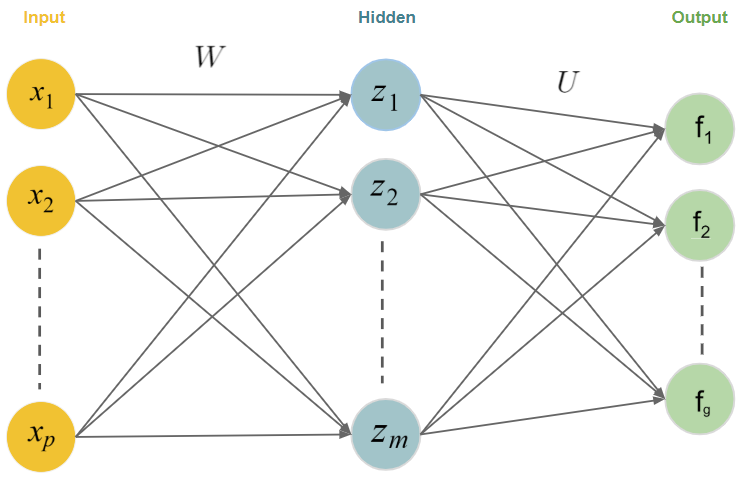
\includegraphics[width=10.2cm]{figure/neuralnet_new.png}}
\caption{\footnotesize Structure of a single hidden layer, feed-forward neural network for g-class classification problems (bias term omitted).}
\end{figure}
\end{itemize}
\end{frame}
%%%%%%%%%%%%%%%%%%%%%%%%%%%%%%%%%%%%%%%%%%%%%%%%%%%%%%%%%%%%%%%%%%

\begin{frame} {Multi-class Classification}
\vspace{5mm}
\begin{blocki}{Notation:}
\item For $g$-class classification, $g$ output units: $$\mathbf{f} = (f_1, \dots, f_g)$$
\vspace{4mm}
\item $m$ hidden neurons $z_1, \dots, z_m$, with
    $$ z_j = \sigma(\mathbf{W}_j^T \xv), \quad j = 1,\ldots,m. $$
\item Compute linear combinations of derived features $z$:
    $$ f_{in,k} = \bm{U}_k^T \hidz, \quad \hidz=(z_1,\dots, z_m)^T, \quad k = 1,\ldots,g$$
\end{blocki}
\end{frame}
%%%%%%%%%%%%%%%%%%%%%%%%%%%%%%%%%%%%%%%%%%%%%%%%%%%%%%%%%%%%%%%%%%

\begin{frame} {Multi-class Classification}
  \begin{itemize}
    \item The second step is to apply a softmax activation function to the output layer.
    \vspace{4mm}
    \item This gives us a probability distribution over $g$ different possible classes:
    $$ f_{out,k} = \tau_k(f_{in,k}) = \frac{\exp(f_{in,k})}{\sum_{k'=1}^g\exp(f_{in,k'})}$$
    \vspace{2mm}
    \item This is the same transformation used in softmax regression!
    \vspace{4mm}
    \item Derivative $ \frac{\partial \tau(\mathbf{f}_{in})}{\partial \mathbf{f}_{in}} = \text{diag}(\tau(\mathbf{f}_{in})) - \tau(\mathbf{f}_{in}) \tau(\mathbf{f}_{in})^T $
    \vspace{4mm}
    \item It is a \enquote{smooth} approximation of the argmax operation,
        so $\tau((1, 1000, 2)^T) \approx (0, 1, 0)^T$ (picks out 2nd element!).
  \end{itemize}
\end{frame}
%%%%%%%%%%%%%%%%%%%%%%%%%%%%%%%%%%%%%%%%%%%%%%%%%%%%%%%%%%%%%%%%%%

\begin{frame} {Multi-class Classification: Example}
Forward pass (Hidden: Sigmoid, Output: Softmax).
  \begin{figure}
    \centering
      \only<1>{\scalebox{0.95}{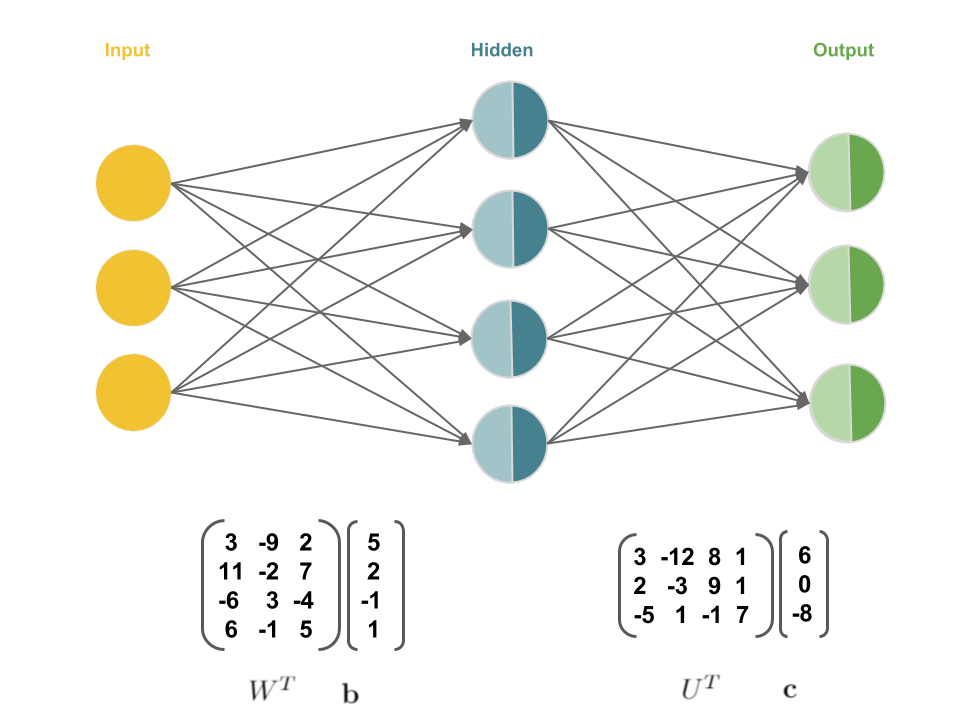
\includegraphics{figure/softie_one.png}}}
      \only<2>{\scalebox{0.95}{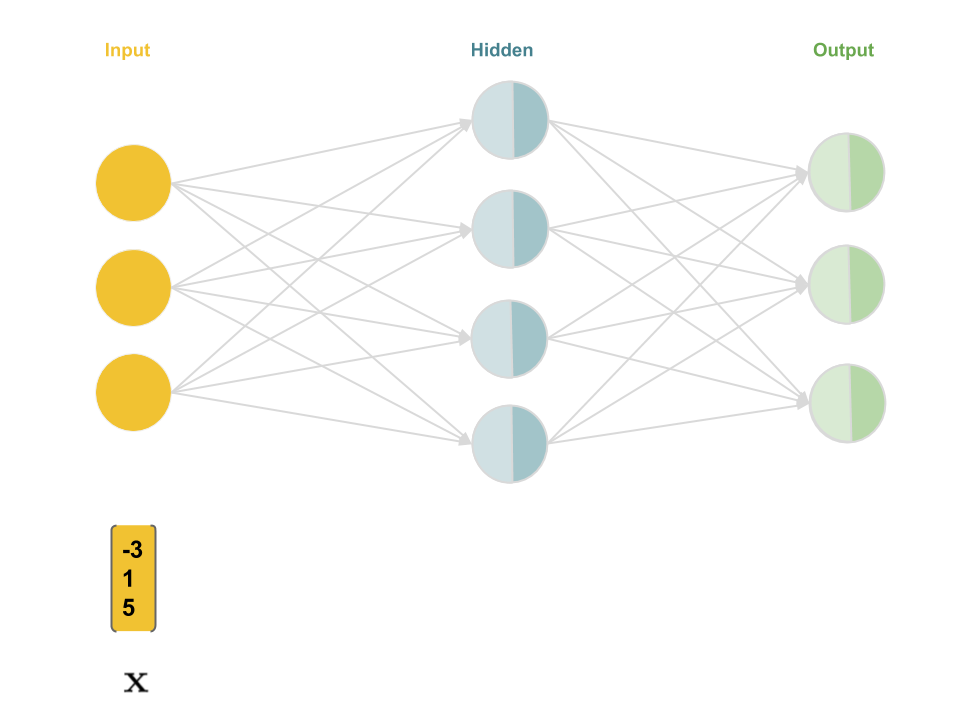
\includegraphics{figure/softie_two.png}}}
      \only<3>{\scalebox{0.95}{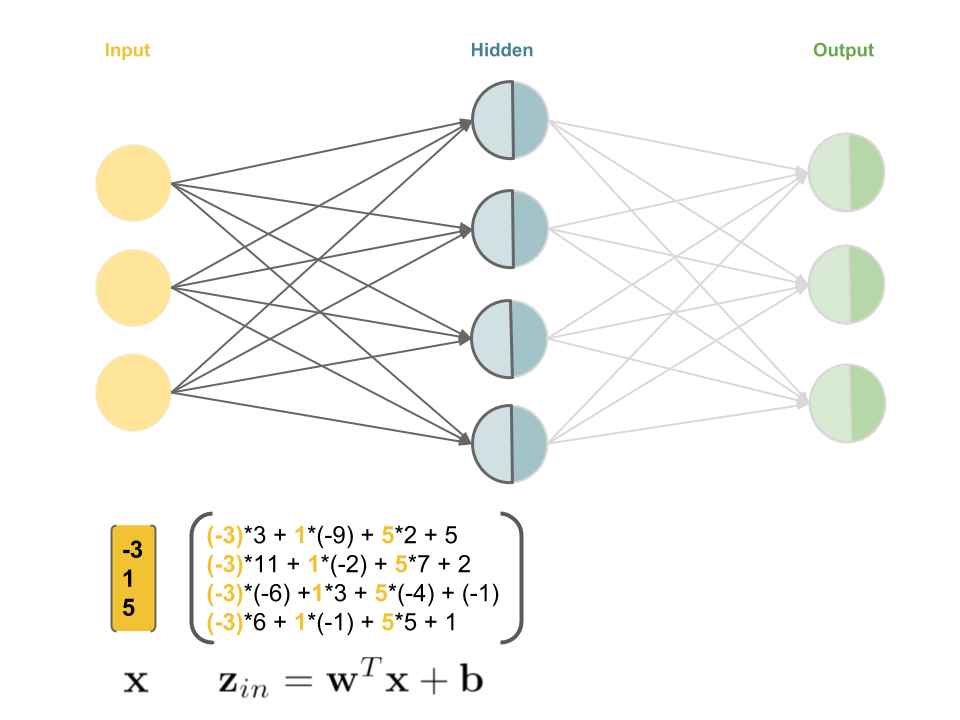
\includegraphics{figure/softie_three.png}}}
      \only<4>{\scalebox{0.95}{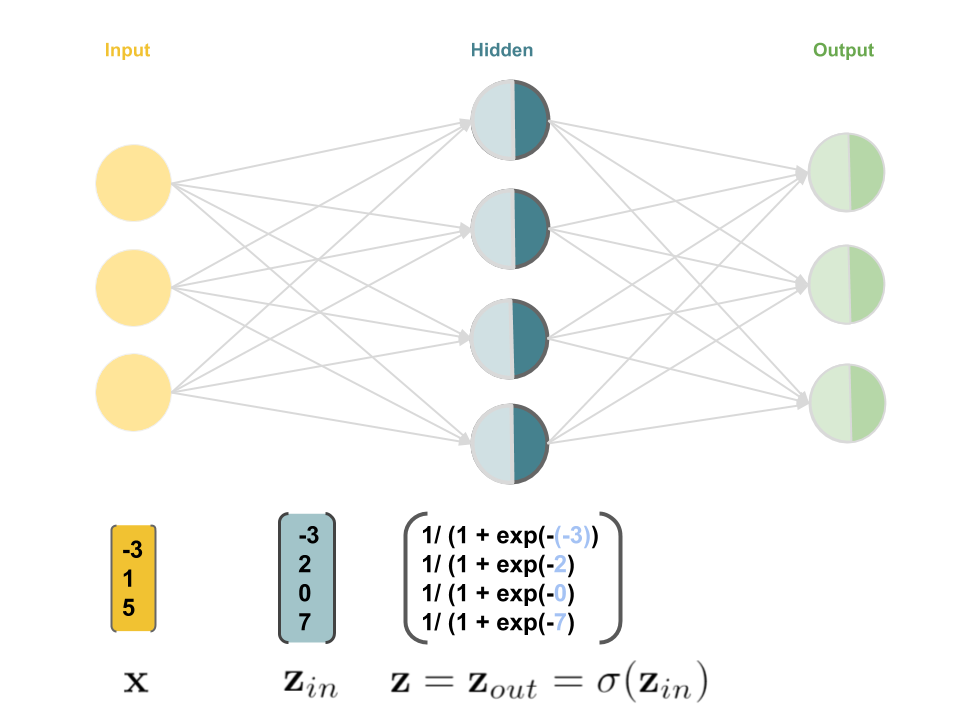
\includegraphics{figure/softie_four.png}}}
      \only<5>{\scalebox{0.95}{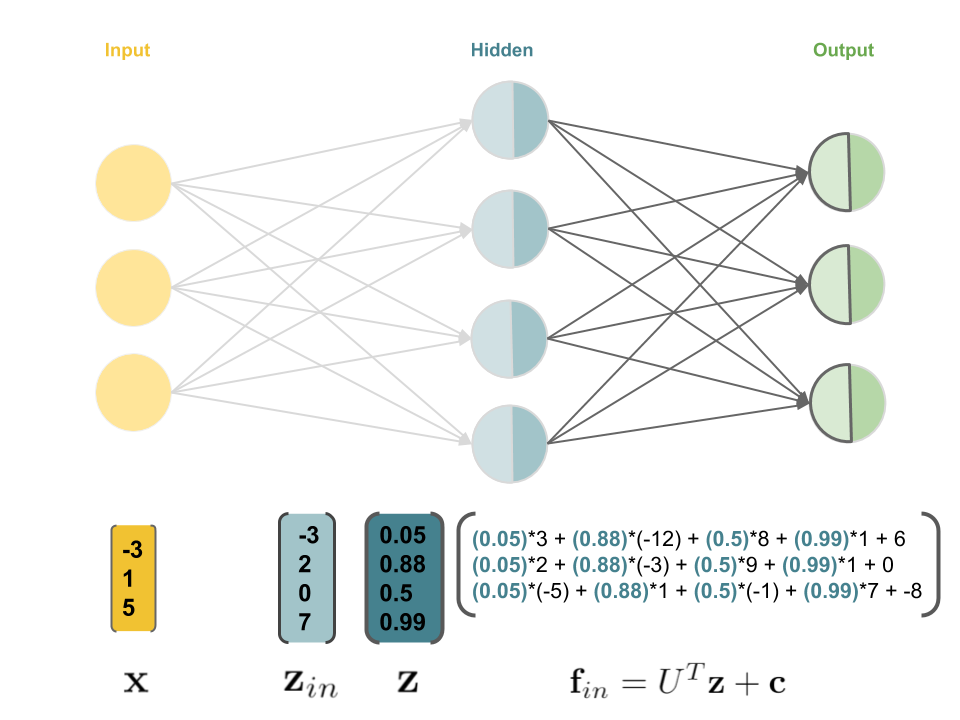
\includegraphics{figure/softie_five_a.png}}}
      \only<6>{\scalebox{0.95}{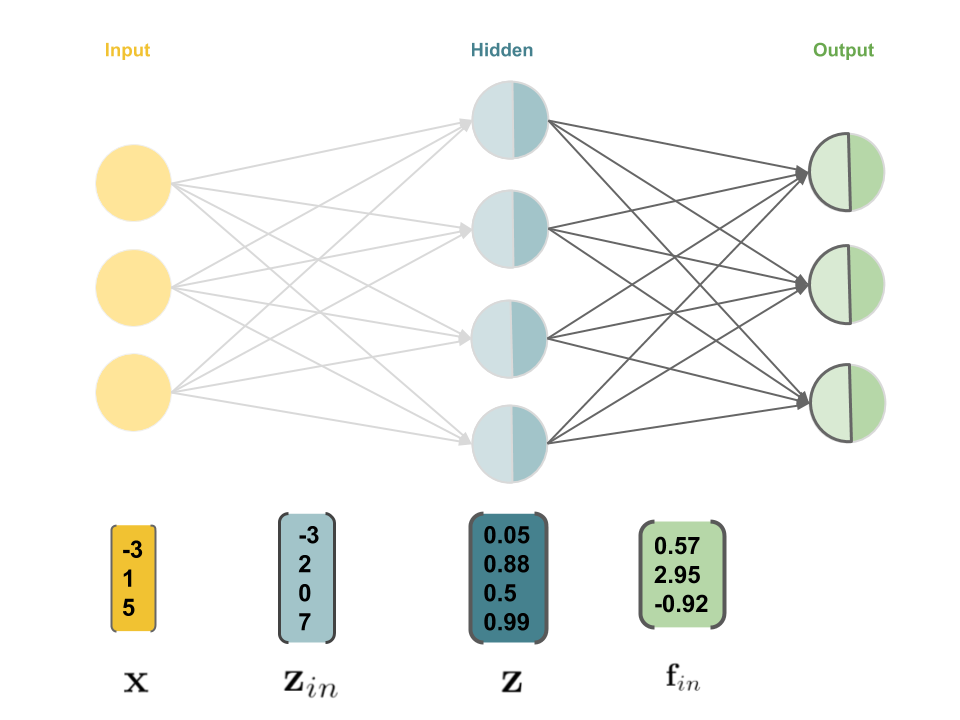
\includegraphics{figure/softie_five_b.png}}}
      \only<7>{\scalebox{0.95}{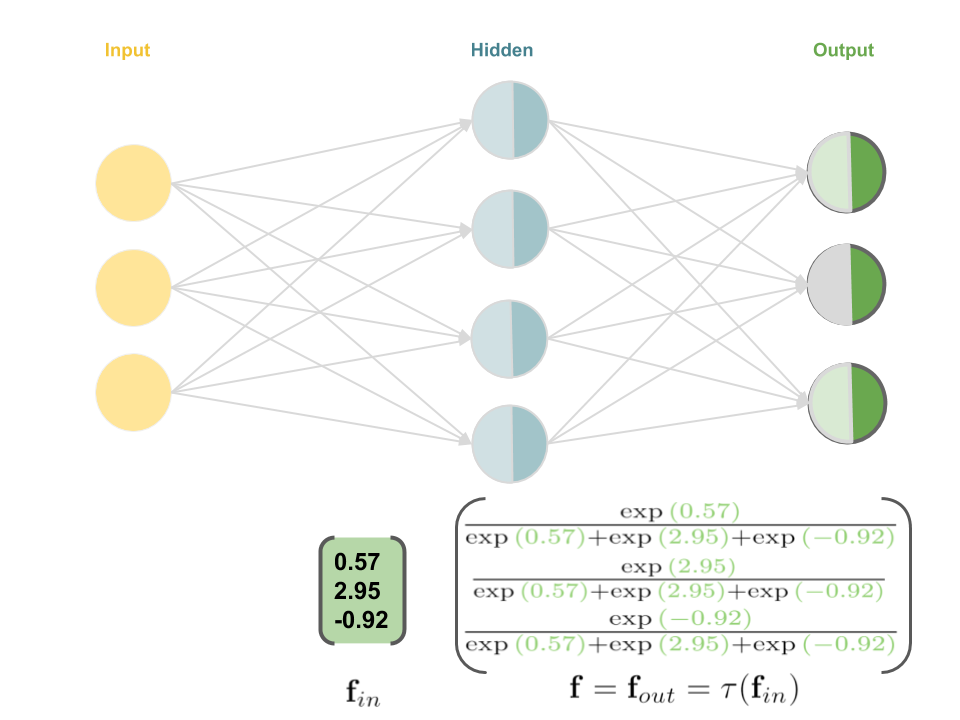
\includegraphics{figure/softie_six.png}}}
      \only<8>{\scalebox{0.95}{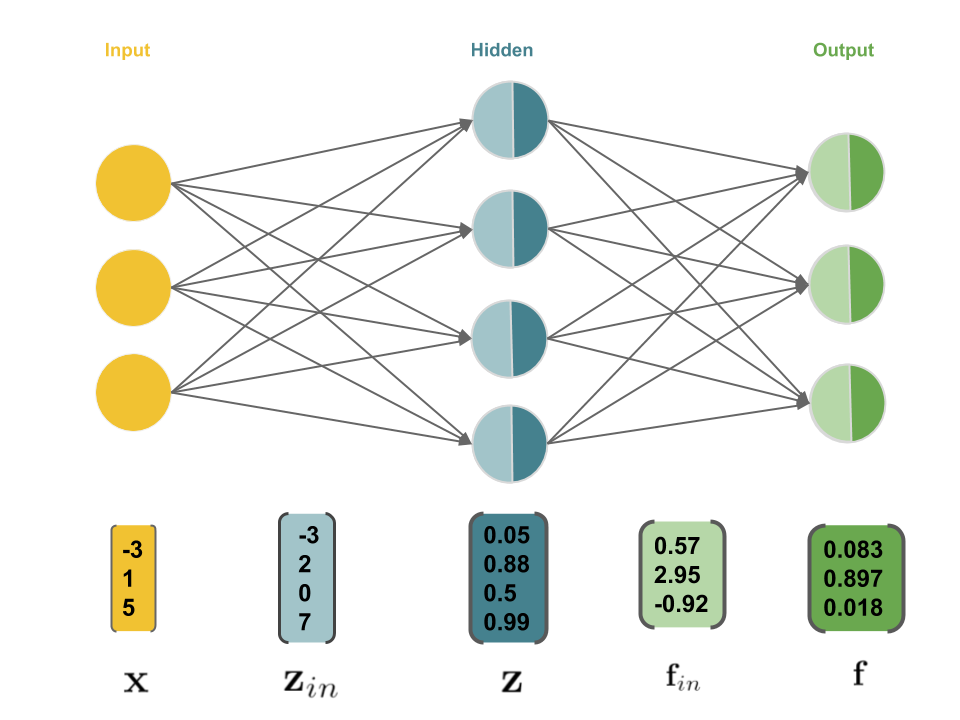
\includegraphics{figure/softie_seven.png}}}
\end{figure}
\end{frame}
%%%%%%%%%%%%%%%%%%%%%%%%%%%%%%%%%%%%%%%%%%%%%%%%%%%%%%%%%%%%%%%%%%

\begin{frame} {Softmax Loss}
  \begin{itemize}
\vspace{5mm}
\item The loss function for a softmax classifier is
$$L(y, \fx) = - \sum_{k = 1}^g [y = k] \log \left( \frac{\exp(f_{in,k})}{\sum_{k'=1}^g\exp(f_{in,k'})}\right)$$
where $[y = k] = \begin{cases} 1 & \text{ if } y = k \\
0 & \text{ otherwise }
\end{cases}$. 
\vspace{5mm}
\item This is equivalent to the cross-entropy loss when the label vector $\bm{y}$ is one-hot coded (e.g. $\mathbf{y} = (0,0,1,0)^T$). 
\item Optimization:  Again, there is no analytic solution.
\end{itemize}
\end{frame}
%%%%%%%%%%%%%%%%%%%%%%%%%%%%%%%%%%%%%%%%%%%%%%%%%%%%%%%%%%%%%%%%%%

\endlecture
\end{document}